\documentclass[12pt,a4paper,openright,dvipsnames]{mwart}

\usepackage{lmodern}
\usepackage[T1]{polski}
\usepackage[utf8]{inputenc}

\usepackage[a4paper,
            tmargin=2cm,
            bmargin=2cm,
            lmargin=2cm,
            rmargin=2cm,
            bindingoffset=0cm]{geometry}

\usepackage{tocloft}
\usepackage{hyperref}

\usepackage{amsmath}
\usepackage{amssymb}
\usepackage{siunitx}

\usepackage{listings}

\usepackage{graphicx}
\usepackage{subfig}
\usepackage{float}
\usepackage{booktabs}

\usepackage{xcolor}


\hypersetup{
    colorlinks,
    citecolor=black,
    filecolor=black,
    linkcolor=black,
    urlcolor=black
}


\newcommand{\vtitle}{ESP32 Synthesizer}
\newcommand{\vauthors}{
    Jakub Karbowski
}


\begin{document}
\begin{titlepage}
    \centering

    \textsc{Akademia Górniczo-Hutnicza im. Stanisława Staszica w Krakowie}

    \vspace{\stretch{1}}

    {\LARGE\bfseries \vtitle\\}
    \rule{3in}{0.4pt} \\
    \today

    \vspace{\stretch{1}}

    \large\vauthors

    \vspace*{\stretch{2}}

\end{titlepage}



\section{Wstęp}

Celem projektu było zbudowanie syntezatora cyfrowego na
platformie ESP32. Syntezator ten ma być w stanie odtwarzać
dźwięki na podstawie komend MIDI, które będą przesyłane
do niego przez port szeregowy.
Taki interfejs pozwala na łatwe połączenie z komputerem lub
keyboardem MIDI.


\subsection{Specyfikacja}

Syntezator ma obsługiwać następujące funkcje:
\begin{enumerate}
    \item dekodowanie pełnego zestawu komend MIDI,
    \item polifonię na przynajmniej 4 głosy,
    \item funkcję ADSR (Attack, Decay, Sustain, Release),
    \item oscylatory piłokształtne,
    \item odtwarzanie dźwięku przez DAC protokołem I2S.
\end{enumerate}


\subsection{Zbudowana platforma}

Użyte komponenty:
\begin{enumerate}
    \item ESP32 DevKitC,
    \item Adafruit UDA1334A I2S DAC,
    \item głośnik, który znalazłem w śmieciach,
    \item wyświetlacz dotykowy z kontrolerem ILI9341,
    \item enkoder obrotowy.
\end{enumerate}

\begin{figure}[h]
    \centering
    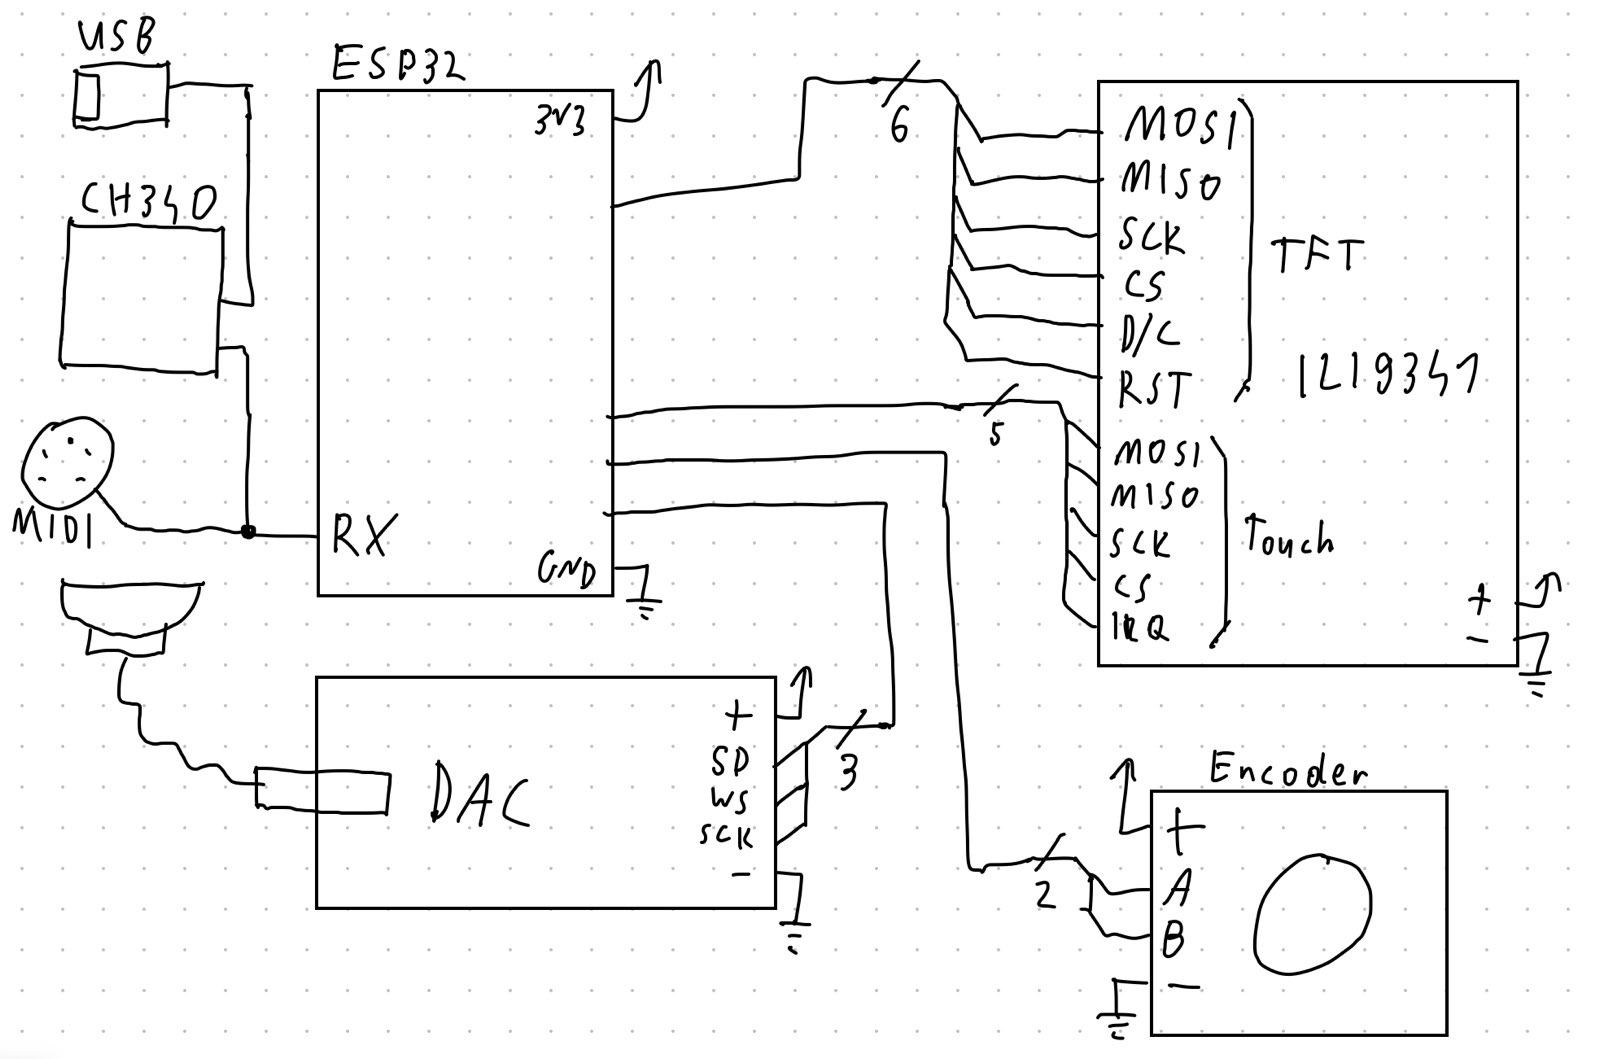
\includegraphics[width=\textwidth]{schem}
    \caption{Schemat urządzenia}
\end{figure}


\section{Wstępne próby}

Początkowo, planem było zbudowanie syntezatora
opartego o system Zephyr OS.

Napotkano następujące problemy:
\begin{enumerate}
    \item słabe wsparcie dla I2S w systemie,
    \item niedziałająca implementacja I2S dla posiadanego mikrokontrolera z rodziny STM32,
    \item niedziałająca implementacja UART z DMA dla posiadanego mikrokontrolera.
\end{enumerate}

Podjęto próby rozwiązania tych problemów.

\subsection{I2S w Zephyr OS}

System stara się udostępnić jednolite API dla każdego mikrokontrolera
na świecie. Jest to niemożliwe. Mikrokontrolery różnią się na tyle,
że wymagają indywidualnego podejścia do swoich podsystemów.

Okazało się, że dla posiadanej płytki rozwojowej, Zephyr
nie włączał DMA używanego przez I2S. Po dodaniu
do device tree definicji kontrolera DMA, program zaczął się
kompilować. Ale nie działał. Brak dokumentacji ani
jakichkolwiek przykładów (czy nikt tego nie używa?)
uniemożliwił uruchomienie I2S.

\subsection{Własna karta I2S na FPGA}

Poddając użycie I2S na Zephyrze, zaimplementowany został
konwerter UART -> I2S na FPGA.
Odbiera on specjalnie zakodowane sample przez port szeregowy
z docelową przepustowością 12.5 Mbit/s
i wysyła je przez I2S.
Zastępuje to wbudowany kontroler I2S w mikrokontrolerze.

Aby użyć zaimplementowanego sprzętu, potrzebny jest
jedynie port szeregowy na mikrokontrolerze z DMA,
aby transfer był szybki i nie blokował procesora
(procesor jest zajęty generowaniem dźwięku).

Niestety, Zephyr strikes again, DMA nie było poprawnie skonfigurowane
na dostępnej płytce i nie działało z UARTem.
Problem był na tyle trudny do debugowania (zero błędów, kodów błędu, po prostu nie działa), że poddano ten pomysł.

\begin{figure}[h]
    \centering
    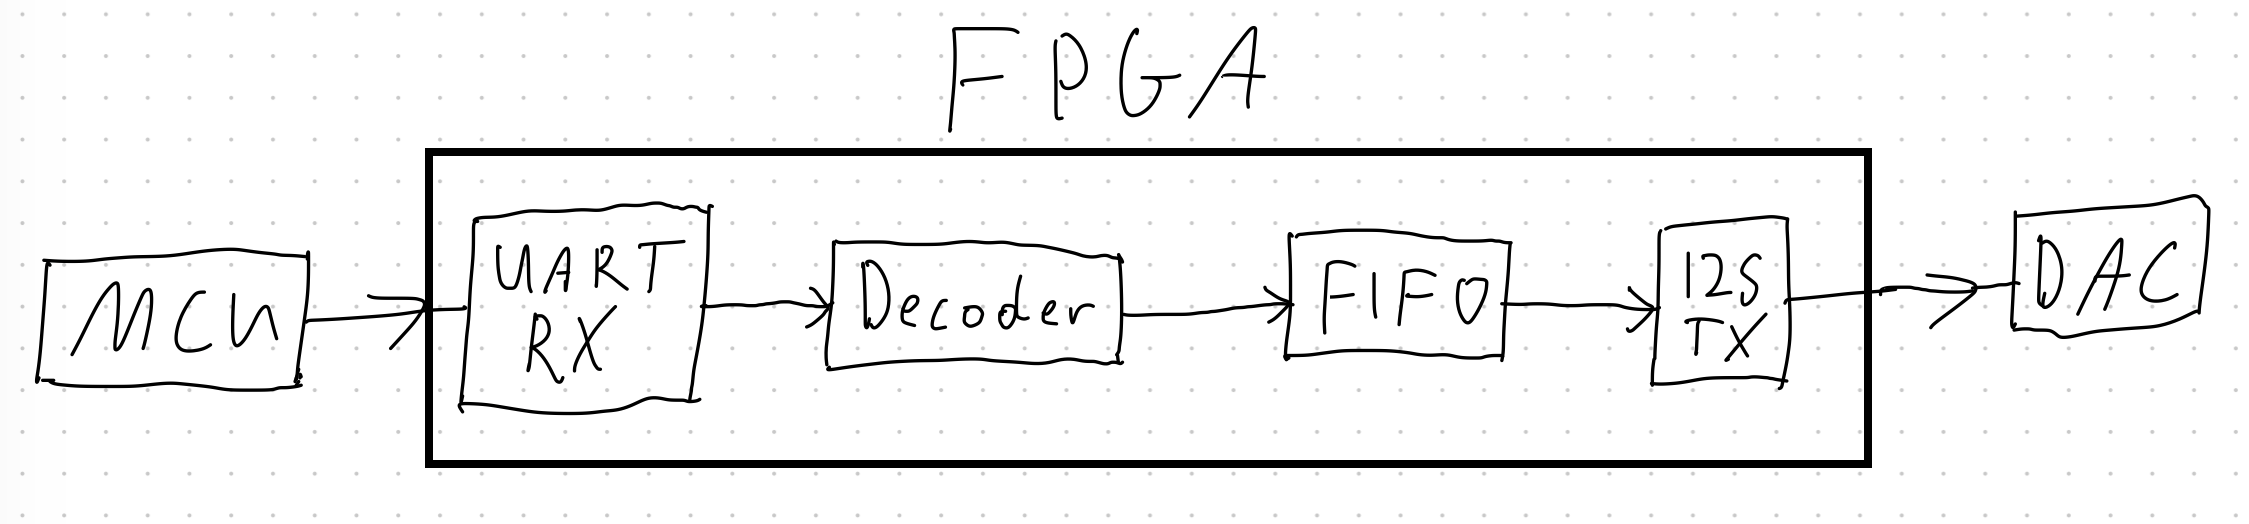
\includegraphics[width=\textwidth]{fpga}
    \caption{Schemat urządzenia FPGA}
\end{figure}

\subsection{Finalna opinia}

Zephyr jest piękny w teorii i zapewne sprawdza się
w wysokopoziomowych systemach IoT, gdzie głównie interesuje
nas komunikacja IP lub różne gotowe peryferia jak wyświetlacze.
Jednak jak chcemy użyć płytki mało popularnej (chińskiego klona)
lub użyć niskopoziomowego peryferium, Zephyr jedynie utrudnia pracę.


\section{Zmiana platformy na ESP32}

Aby uniknąć dalszych problemów, wybrano dojrzałą
i dobrze wspieraną platformę ESP32.
Wstępnie planowano zaimplementować urządzenie MIDI
jako USB Device Class. Niestety, ESP32 nie posiada
kontrolera USB i taka implementacja jest niemożliwa.

Zamiast tego, postawiono na kompatybilność i wybrano zwykły
UART do komunikacji MIDI.
Takie rozwiązanie ma swoje plusy.
Pozwala na podłączenie dowolnego rzeczywistego
keyboardu przez port MIDI.


\section{Architektura systemu}

Na ESP32 uruchomiony jest system FreeRTOS.
Własne oprogramowanie składa się z następujących modułów:
\begin{enumerate}
    \item generator dźwięku,
    \item odbiornik MIDI,
    \item sterownik UI,
    \item sterownik pokrętła głośności.
\end{enumerate}

Moduły te komunikują się przez swoje publiczne API.
Ich wewnętrzna implementacja (taski, synchronizacja)
jest ukryta. Publiczne API zapewnia thread safety.

\begin{figure}[h]
    \centering
    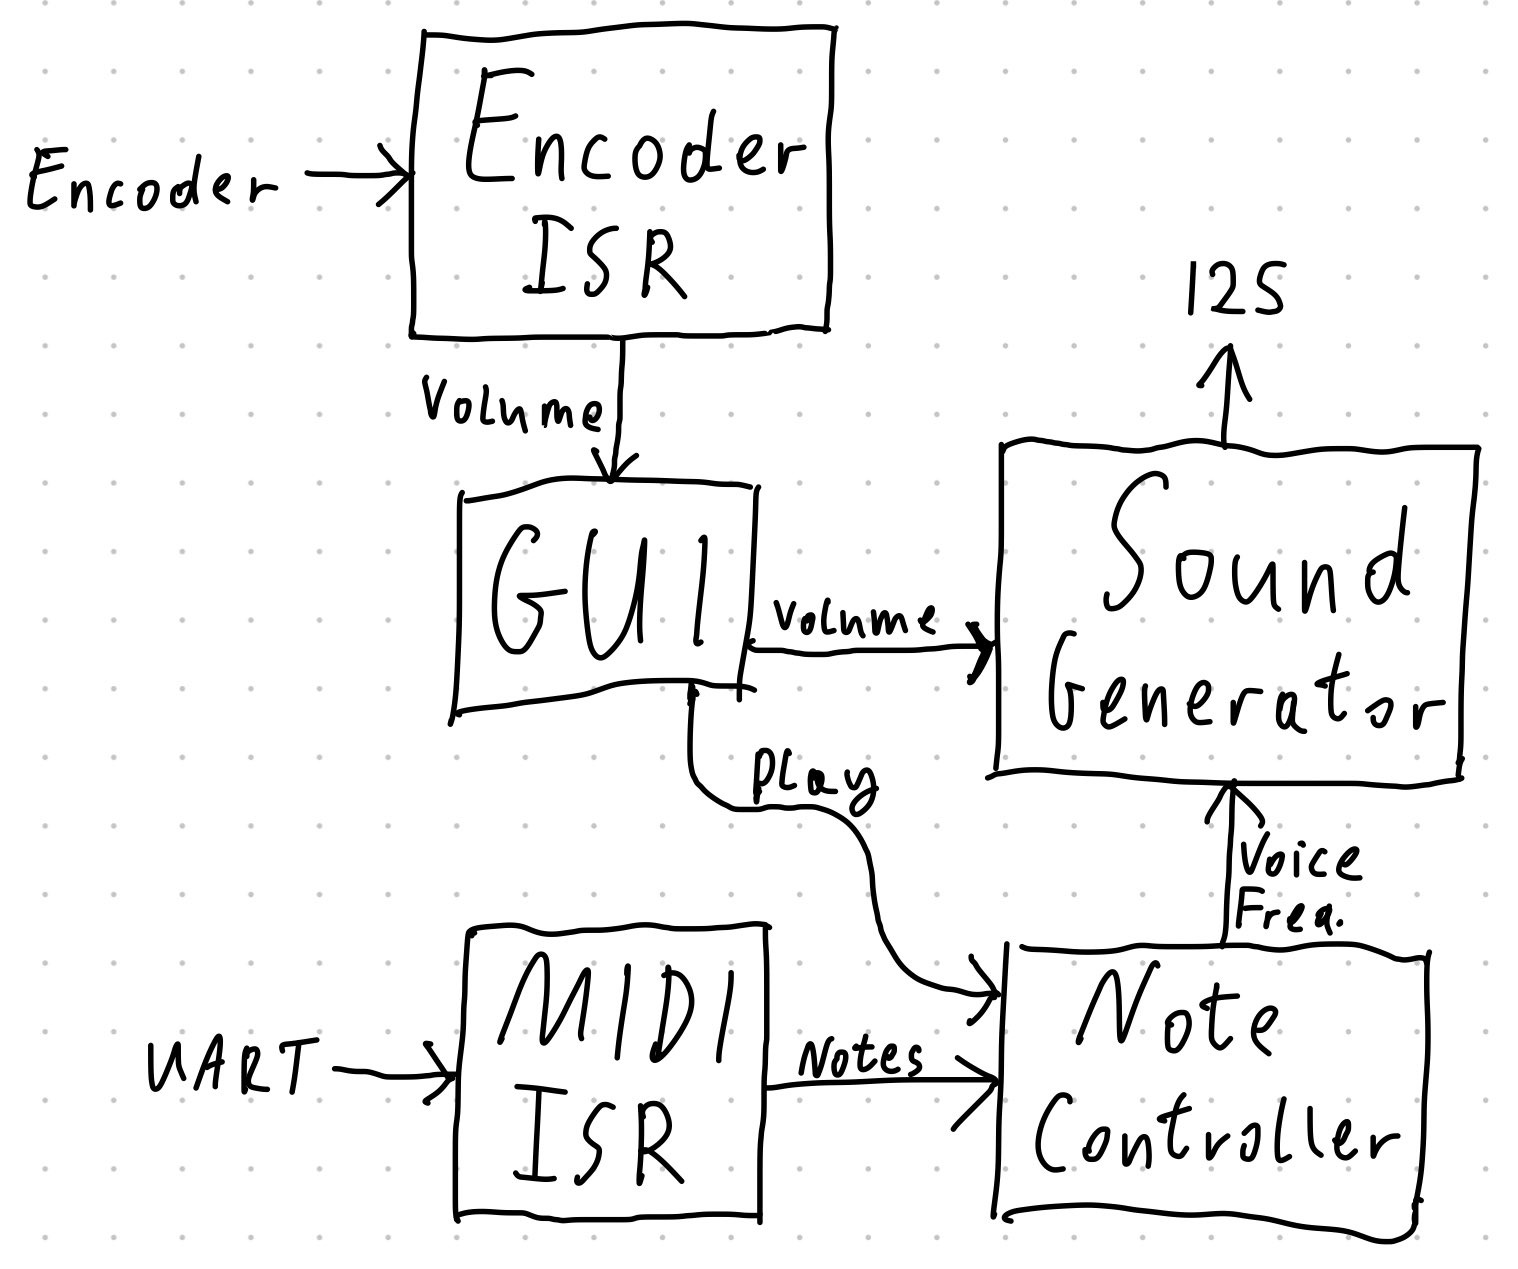
\includegraphics[width=\textwidth]{rtos}
    \caption{Architektura systemu}
\end{figure}


\subsection{Generator dźwięku}

Główny element syntezatora to polifoniczny generator dźwięku.
Główne cechy:
\begin{enumerate}
    \item oscylatory piłokształtne metodą poly blep,
    \item 8-głosowa polifonia,
\end{enumerate}

Oscylatory korzystają z metody poly blep,
co zmniejsza efekt aliasingu.
Oscylatory używane są w obiektach Voice,
które dodają funkcję ADSR.
Wiele Voice łączone jest w jeden obiekt
Syntezatora.

Algorytm schedulingu dźwięków bazuje na
rzeczywistym syntezatorze firmy Korg.
W danej chwili, z pośród wszystkich zarządanych dźwięków,
odtwarzane jest $n$ najwyższych.
Opiera się to na założeniu, że melodia zwykle jest grana
na wyższych dźwiękach, a niższe dźwięki są trudniejsze
do usłyszenia.
Rozwiązanie sprawdza się bardzo dobrze.

Odtwarzanie przez I2S wykorzystuje autorską
bibliotekę do ESP-IDF.
Ułatwia ona tworzenie aplikacji grających,
konfigurując wyjście I2S i
tworząc wątek przetwarzania dźwięku.
Biblioteka przyjmuje callback od użytkownika
do generacji jednego buffera sampli audio.

Moduł generatora dźwięku udostępnia funkcje
do naciśnięcia i puszczenia klawiszy.



\subsection{Odbiornik MIDI}

Moduł MIDI to autorska biblioteka do ESP-IDF.
Wykorzystuje ona przerwania wysokiego priorytetu
i bezpośredni dostęp do peryferium UART,
dzięki czemu minimalizuje opóźnienia.

Biblioteka rejestruje przerwanie odebrania znaku przez UART.
W funkcji obsługi przerwania wykonywane jest parsowanie
komend MIDI. Wspierany jest pełny zestaw komend.
Po zdekodowaniu wielu bajtów do pakietów MIDI,
przerwanie wysyła gotowy pakiet kolejką FreeRTOS
do osobnego wątku. Wątek ten wykonuje callback użytkownika,
dzięki czemu możliwe jest wykonanie dowolnych funkcji.


\subsection{Sterownik UI}

UI wyświetlane jest na dotykowym ekranie RGB
ze sterownikiem ILI9341.
Wykorzystana została biblioteka LVGL.
Jest to duży framework do tworzenia interaktywnych aplikacji,
z obsługą animacji i gestów dotykowych. Zawiera ona
wiele przydatnych elementów budowy UI jak guźiki, suwaki.

Interfejs zawiera:
\begin{enumerate}
    \item przycisk Mute -- ustaw głośność 0\%,
    \item przycisk Play Note -- zagraj przykładowy dźwięk,
    \item suwak głośności -- głośność od 0\% do 100\%,
    \item indykator numeryczny poziomu głośności.
\end{enumerate}

Użytkownik może sterować poziomem głośności syntezatora
za pomocą suwaka.
Stan suwaka oraz Label pokazujący poziom głośności
jest synchronizowany z drugim źródłem głośności, czyli enkoderem.



\subsection{Sterownik pokrętła głośności}

Pozwala on na wygodne sterowanie głośnością.
Jest on synchronizowany z poziomem głośności
na wyświetlaczu (enkoder -> UI).

Enkoder wykorzystuje przerwanie na jednym z pinów.
Przerwanie reaguje na dowolną krawędź sygnału.
Na krawędzi sygnału A sprawdzany jest sygnał B,
który decyduje o kierunku obrotu.



\section{Efekty}

Projekt napotkał wiele problemów, jednak udało się
zrealizować cel dzięki zmianie platformy.

\begin{enumerate}
    \item syntezator jest w stanie odtwarzać melodie z komputera,
    \item pozwala na podłączenie zewnętrznego urządenia MIDI,
    \item jakość generowanego dźwięku jest zadowalająca i pozwala
    na odtwarzanie zaawansowanych utworów,
    \item renderowanie interfejsu i obsługa dotyku nie wpływa na generację
    dźwięku, dzięki wielordzeniowości procesora,
    \item UI jest responsywne, atrakcyjne i użyteczne,
    \item pokazana została integracja fizycznego pokrętła
    z wirtualnym suwakiem,
\end{enumerate}


\section{Wnioski}

System ZephyrOS jest jeszcze bardzo młody i ciągle się rozwija.
Autorzy postawili na wspieranie jak największej liczby MCU,
przez co wsparcie każdego z nich jest na niskim poziomie
(blink zazwyczaj działa).

Podejście ,,jedno API do każdego sprzętu'' budzi wątpliwości.
Powoduje to, że dużo funkcji pewnych mikrokontrolerów nie jest
dostępna (np SAI na STM32), bo Zephyr nie definiuje API do
sprzętu tej klasy.

ESP32 z frameworkiem ESP-IDF znowu okazało się dopracowane
i dobrze wspierane (już sprawdziło się w poprzednich projektach).
Dobra dokumentacja, aktywne społeczeństwo i sprawdzony RTOS
powodują, że implementacja swojego pomysłu jest bezproblemowa.

Było to moje pierwsze spotkanie z biblioteką LVGL.
Do uruchomienia wymaga ona sporej liczby boilerplate
kodu, ale po uruchomieniu jest bardzo wygodna w użyciu.
Interfejs graficzny działa bardzo płynnie.
Sterowanie dotykiem jest proste w użyciu i implementacji
(LVGL automatycznie wykrywa naciśnięte elementy).

Zbudowany syntezator działa dobrze.

\begin{figure}[h]
    \centering
    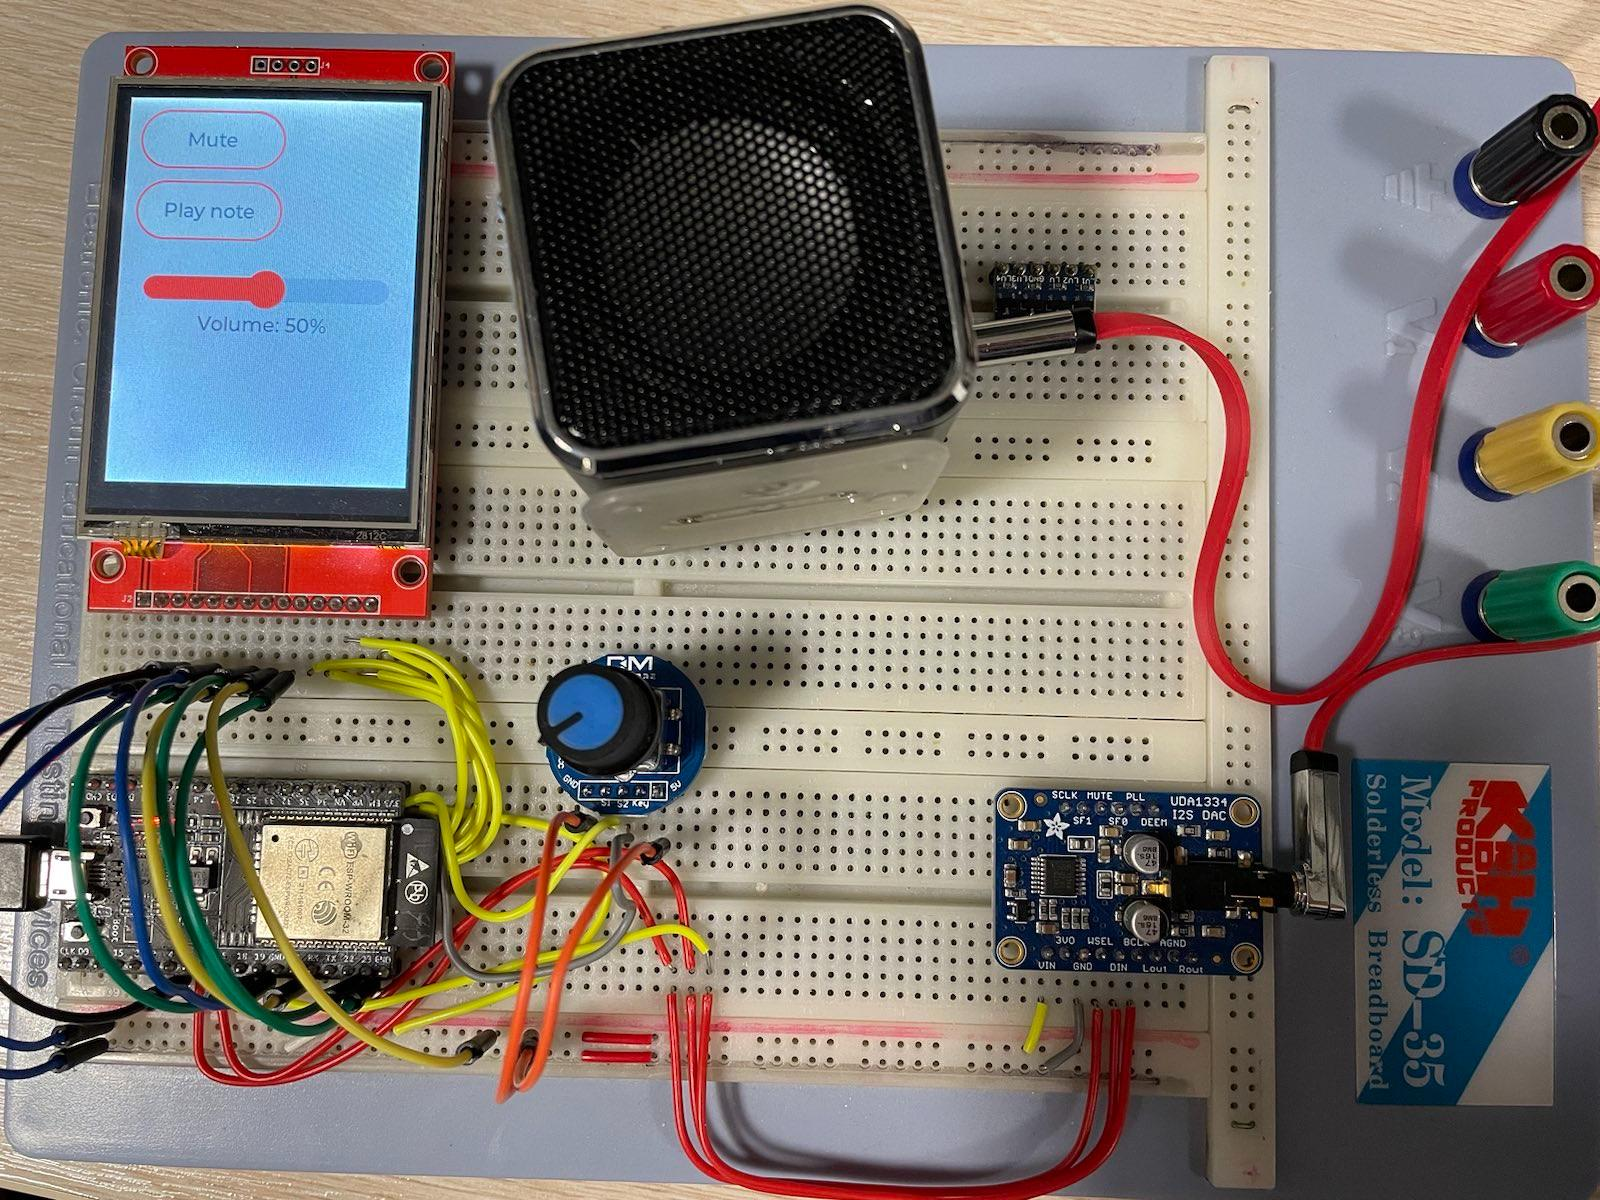
\includegraphics[width=0.8\textwidth]{synth}
\end{figure}




\end{document}
